\subsubsection{Combustor Material Study}

The chamber of an RDE contains the inner body, the outer body, the annulus gap, and any interfaces with diagnostic instrumentation, injectors, plenums, and the nozzle/aerospike. The material selection for this assembly is very important as the hot gases flowing through the annulus will reach temperatures and pressures around 3000K and 1600psi (11 MPa). With increased temperature, the yielding strength of materials greatly decreases. Additionally, materials tend to oxidate much more rapidly when exposed to high temperature combustion. 

A trade study was conducted to determine the ideal chamber material for the SABR system dependent upon the cost, schedule, risk, manufacturability, and technical performance. It considered Copper and 304 Stainless Steel, as recommended by industry professionals. The relevant requirements were derived and reported to assist in contextualizing this trade study, Next, evaluation criteria were decided based on the factors that affect the success of the system, project functions, and safety of operators. Then, the evaluation scales and weights were determined based on their expected effects on the same factors used to define the evaluation criteria. Measures of Performance were defined to induce a scientific approach to the technical performance scoring. Finally, each option was evaluated and input into a decision matrix, where an optimal material was defined.

\noindent\underline{Option 1: Copper 110}

\noindent\textit{Pros:}

Copper is often used for combustion chambers due to its heat sink capabilities. This is a function of its thermal conductivity. During operation, copper’s high thermal conductivity (about 400 W/m-K) allows heat to be transferred at a high rate from the inner surface to the outer surface. Thus, active cooling methods can be maximized. Additionally, cooling after operation can be maximized with a high thermal conductivity due to a higher heat transfer rate than materials with a lower thermal conductivity. 

The common availability of copper also contributes to its favorability. If any roadblocks introduce themselves during procurement, it is important to pivot to alternative vendors. Copper stock can be delivered within one week of purchase.

Due to copper’s low rating on the hardness scales, expensive tooling is not required; however, it can be damaged due to its high ductility. This opens the opportunity for mistakes during manufacturing, integration, and testing processes. These risks are much less impactful than a material that ranks high on the hardness scale, though.

\noindent\textit{Cons:}

Copper’s high price compared to other commonly available metals may make its acquisition infeasible. The group currently possesses a quote for one foot of 4-inch-diameter copper stock for about \$550. Under the assumption that the group would receive \$1,000 in funding, the procurement of this material would severely impact the budget available for the other systems and components.

Also, copper’s yield strength at high temperatures is potentially a cause for concern. The yield strength of pure copper at room temperature is about 70 MPa, but it decreases greatly with temperature as seen in Figure \ref{fig:metallic-materials-strength}. Given that the nominal conditions are expected to be about 11 MPa, other material options should be considered. It is still a viable option as prior work has demonstrated that this effect is negligible for short duration tests; however, more research must be done to be sure of its passing of yield strength under nominal conditions.

\begin{figure}
    \centering
    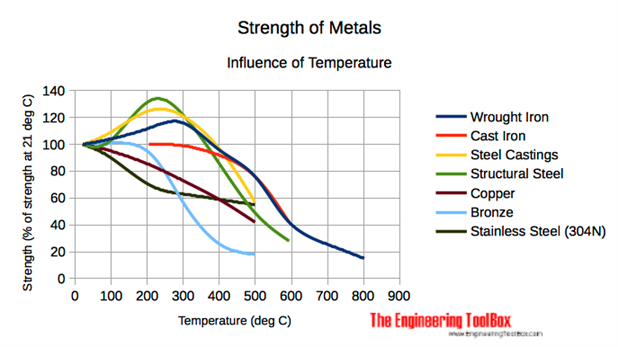
\includegraphics[width=0.8\linewidth]{metallic_materials_strength.png}
    \caption{Strength of metallic materials as a function of temperature.}
    \label{fig:metallic-materials-strength}
\end{figure}

The melting point of copper is about 1400 K. The expected nominal conditions are at about 3000 K. Thus, alternative material options should be considered. Prior work has shown that this is negligible for short duration tests, though. This concern may be mitigated with the use of regenerative cooling, but the inclusion of such design introduces additional complexity to the systems and integration.

The technical performance of copper in the application of our system can be characterized by its thermal conductivity, yield strength at nominal temperature, melting point, and indentation hardness on the Rockwell B scale. It performs very well in thermal conductivity, but it lacks the ability to withstand operational pressures and temperatures on its own. The use of this material for the combustor will lean on the external sources of cooling as is common in liquid rocket engines. This capability has been proven in adjacent engine configurations, and there is current work in the industry to realize this cooling method for RDEs.

\noindent\underline{Option 2: 304 Stainless Steel}

\noindent\textit{Pros:}

Stainless steel is attractive as a material option mainly due to its low cost. For a 4-inch diameter and 14 in. in length stock of 304 Stainless Steel, it costs about \$200. The procurement of this material would allow more expensive purchases in other systems. Also, if more stock needs to be ordered, the price will not be too detrimental to the outcome of the project.

304 Stainless Steel has a yield strength of 215 MPa. It also has a nominal yield strength of 75 MPa at 1170K. This is much higher than the operating pressure of 11 MPa, and thus is a viable option for medium duration run time (greater than 1 second but less than 10 seconds). This capability would be helpful in testing the time effects on operational capability.

Additionally, 304 Stainless Steel has a melting point of about 1725K. This would potentially contribute to higher operational times without the need for complex cooling systems. It can also help increase the amount of test cases for short duration runs.

\noindent\textit{Cons:}

304 Stainless Steel is not great for cooling, though. It has a thermal conductivity of 21.5 W/m-K. Thus, regenerative cooling would be fairly infeasible with non-cryogenic fluids. However, cooling may not be necessary for our operational setting with the high melting point and high yield stress of this material.

Another drawback of 304 Stainless Steel is the challenges with machining. It has a high work hardening rate, which requires machining procedures to be much more precise. However, this high strength means that ductility effects during machining won’t be as much of a concern.

Finally, 304 Stainless Steel tends to oxidate at high temperatures when working with pure oxygen. However, when using higher Nitrogen percentages, this concern becomes negligible. This limits our operational conditions to a range of nitrogen dilution close to and including that of air.

The technical performance of 304 Stainless Steel in the application of our system can be characterized by its thermal conductivity, yield strength at nominal temperature, melting point, and indentation hardness on the Rockwell B scale. It performs fairly well in all categories except for thermal conductivity. The use of this material for the combustor will lean on the ability to withstand pressures and temperatures rather than external sources of cooling. This capability has been proven in heritage systems and will leverage their design approaches.

% ----- CRITERIA & WEIGHTS -----
\begin{table}[H]
    \centering
    \singlespacing
    \small
    \caption{Combustor Material Trade Study - Evaluation Criteria}
    \label{tab:combustor_material_eval_criteria}

    \begin{subtable}[t]{\linewidth}
        \begin{tabularx}{\linewidth}{
            |>{\hsize=0.200\hsize}>{\centering\arraybackslash}X
            |>{\hsize=0.100\hsize}>{\centering\arraybackslash}X
            |>{\hsize=0.700\hsize}>{\centering\arraybackslash}X|
        }
            \hline
            \textbf{Decision Criteria} & \textbf{Weight} & \textbf{Reason} \\ \hline

            Cost & 30\% & The combustion chamber is one of many components included in SABR. Thus, the cost of this assembly must be as low as possible while meeting proper performance standards. \\ \hline
        
            Schedule & 10\% & The lead time necessary for stock must be as low as possible to start machining the components as soon as possible. This will allow proper time for integration and V\&V events. \\ \hline
        
            Risk & 15\% & This component should not introduce significant risk for the operation of SABR. \\ \hline

            Manufacturability & 15\% & The ease of manufacturing will allow a shorter lead time on machining and mitigate accidents during those processes \\ \hline
        
            Technical Performance & 25\% & The material chosen for the combustion chamber must withstand operational conditions. \\ \hline
        \end{tabularx}
        \smallskip
        \caption{Evaluation Criteria and Weights}
    \end{subtable}

\end{table}

\vspace{-2em}

% ----- COST SCALE -----
\begin{table}[H]
    \centering
    \singlespacing
    \small
    \ContinuedFloat

    \begin{subtable}[t]{0.5\linewidth}
        \begin{tabularx}{\linewidth}{
            |>{\hsize=0.250\hsize}>{\centering\arraybackslash}X
            |>{\hsize=0.750\hsize}>{\centering\arraybackslash}X|
        }
            \hline
            \textbf{Score} & \textbf{Reason} \\ \hline
            
            5 & \$0 - \$100 \\ \hline
            4 & \$100 - \$200 \\ \hline
            3 & \$200 - \$300 \\ \hline
            2 & \$300 - \$400 \\ \hline
            1 & \$400 and above \\ \hline
        \end{tabularx}
        \smallskip
        \caption{Evaluation Scale - Cost}
    \end{subtable}
\end{table}

\vspace{-2em}

% ----- SCHEDULE SCALE -----
\begin{table}[H]
    \centering
    \singlespacing
    \small
    \ContinuedFloat

    \begin{subtable}[t]{0.5\linewidth}
        \begin{tabularx}{\linewidth}{
            |>{\hsize=0.250\hsize}>{\centering\arraybackslash}X
            |>{\hsize=0.750\hsize}>{\centering\arraybackslash}X|
        }
            \hline
            \textbf{Score} & \textbf{Reason} \\ \hline
            
            5 & 0 - 1 week \\ \hline
            4 & 1 - 2 weeks \\ \hline
            3 & 2 - 3 weeks \\ \hline
            2 & 3 - 4 weeks \\ \hline
            1 & 4 weeks and longer \\ \hline
        \end{tabularx}
        \smallskip
        \caption{Evaluation Scale - Schedule}
    \end{subtable}
\end{table}

\vspace{-2em}

% ----- RISK SCALE -----
\begin{table}[H]
    \centering
    \singlespacing
    \small
    \ContinuedFloat

    \begin{subtable}[t]{0.8\linewidth}
        \begin{tabularx}{\linewidth}{
            |>{\hsize=0.150\hsize}>{\centering\arraybackslash}X
            |>{\hsize=0.850\hsize}>{\centering\arraybackslash}X|
        }
            \hline
            \textbf{Score} & \textbf{Reason} \\ \hline
        
            5 & Does not pose any threat \\ \hline
            4 & Does not pose any threat if mitigated measures are in place \\ \hline
            3 & Poses some threat if mitigated measures are in place \\ \hline
            2 & Poses significant threat when mitigations are in place \\ \hline
            1 & Threats are not able to be mitigated \\ \hline

        \end{tabularx}
        \smallskip
        \caption{Evaluation Scale - Risk}
    \end{subtable}
\end{table}

\vspace{-2em}

% ----- MANUFACTURABILITY SCALE -----
\begin{table}[H]
    \centering
    \singlespacing
    \small
    \ContinuedFloat

    \begin{subtable}[t]{0.8\linewidth}
        \begin{tabularx}{\linewidth}{
            |>{\hsize=0.150\hsize}>{\centering\arraybackslash}X
            |>{\hsize=0.850\hsize}>{\centering\arraybackslash}X|
        }
            \hline
            \textbf{Score} & \textbf{Reason} \\ \hline
        
            5 & Very easily manufactured \\ \hline
            4 & Easily manufactured \\ \hline
            3 & Manufactured with some difficulty \\ \hline
            2 & Difficult to manufacture \\ \hline
            1 & Not able to be manufactured at UCF \\ \hline

        \end{tabularx}
        \smallskip
        \caption{Evaluation Scale - Manufacturability}
    \end{subtable}
\end{table}

\vspace{-2em}

% ----- TECHNICAL PERFORMANCE SCALE -----
\begin{table}[H]
    \centering
    \singlespacing
    \small
    \ContinuedFloat

    \begin{subtable}[t]{0.8\linewidth}
        \begin{tabularx}{\linewidth}{
            |>{\hsize=0.150\hsize}>{\centering\arraybackslash}X
            |>{\hsize=0.850\hsize}>{\centering\arraybackslash}X|
        }
            \hline
            \textbf{Score} & \textbf{Reason} \\ \hline
        
            5 & Well withstands operational conditions \\ \hline
            4 & Withstands above operational conditions \\ \hline
            3 & Withstands operational conditions \\ \hline
            2 & Withstands operational conditions at low run times \\ \hline
            1 & Will not withstand operational conditions at low run times \\ \hline

        \end{tabularx}
        \smallskip
        \caption{Evaluation Scale - Technical Performance}
    \end{subtable}
\end{table}

\vspace{-2em}

% ----- DECISION MATRIX -----
\begin{table}[H]
    \centering
    \singlespacing
    \small
    \begin{tabularx}{0.8\linewidth}{
        |>{\hsize=0.35\hsize}>{\centering\arraybackslash}X
        |>{\hsize=0.15\hsize}>{\centering\arraybackslash}X
        |>{\hsize=0.25\hsize}>{\centering\arraybackslash}X
        |>{\hsize=0.25\hsize}>{\centering\arraybackslash}X|
    }
        \hline
        \multicolumn{2}{|c|}{\textbf{Criteria and Weights}} & \multicolumn{2}{|c|}{\textbf{Options and Scores}} \\ \hline

        \textbf{Criteria} & \textbf{Weights} & \textbf{Copper 110} & \textbf{304 St. Steel} \\ \hline

        \multicolumn{1}{|l|}{\textbf{Cost}} & 0.30 & 1 & 3 \\ \hline

        \multicolumn{1}{|l|}{\textbf{Schedule}} & 0.10 & 4 & 4 \\ \hline

        \multicolumn{1}{|l|}{\textbf{Risk}} & 0.15 & 4 & 4 \\ \hline

        \multicolumn{1}{|l|}{\textbf{Manufacturability}} & 0.15 & 4 & 3 \\ \hline

        \multicolumn{1}{|l|}{\textbf{Technical Performance}} & 0.25 & 1 & 3 \\ \Xhline{2pt}

        \multicolumn{2}{|l|}{\textbf{Weighted Scores}} & \textbf{2.15} & \textbf{3.35} \\ \hline
        
    \end{tabularx}
    \caption{Combustor Material Trade Study - Decision Matrix}
    \label{tab:combustor_material_decision_matrix}
\end{table}